\documentclass{vegapresentation}

\DeclareMathOperator*{\cor}{\operatorname{corr}}


\subtitle{Student Research Group 'Stochastic Volatility Models'}
\title{Methods of Simulation of the Heston Model: A Review}
\author{Artemy Sazonov, Danil Legenky, Kirill Korban}
\institute{Lomonosov Moscow State Univesity, Faculty of Mechanics and Mathematics}
\begin{document}
    \maketitle

    \begin{frame}{Heston Model Definition}
        Assume that the spot asset at time $t$ follows the diffusion
        \begin{align}
            dS(t) & = \mu S(t)dt + \sqrt{v(t)} S(t) dZ_1(t), \label{Heston:price}\\
            dv(t) & = \left(\delta^2 - 2\beta v(t)\right) dt + 2\delta \sqrt{v(t)} dZ_2(t), \label{Heston:variance}
        \end{align}
        where $Z_1$, $Z_2$ are the correlated Wiener processes with $dZ_1dZ_2 = \rho dt$.
    \end{frame}

    \section{Introduction to Monte-Carlo Methods}
        \chapter{A review of the original Heston model}
    \section{Basic facts}
        We shall use the following resources in this chapter: \cite{Heston1993} and \cite{Gatheral2012}.
        Assume that the spot asset's price $S$ at time $t$ follows the diffusion \eqref{Heston:price} -- \eqref{Heston:variance}:
        \begin{align}
            dS(t) & = \mu S(t)dt + \sqrt{v(t)} S(t) dZ_1(t), \label{Heston:price}\\
            dv(t) & = \left(\delta^2 - 2\beta v(t)\right) dt + 2\delta \sqrt{v(t)} dZ_2(t), \label{Heston:variance}
        \end{align}
        where $Z_1$, $Z_2$ are the correlated Wiener processes with $dZ_1dZ_2 = \rho dt$.
    \section{PDEs}
    \section{A closed-form solution for the European call option}
\chapter{A review of the Monte-Carlo methods for diffusions}
    \section{Randomness in Probability Theory}
        A. N. Kolmogorov in <<On Logical Foundations of Probability Theory>>: 
        
        \textit {In everyday language we call random these phenomena where we cannot find a regularity allowing us to predict precisely their results. Generally speaking there is no ground to believe that a random phenomenon should possess any definite probability. Therefore, we should have distinguished between randomness proper
        (as absence of any regularity) and stochastic randomness (which is the subject of the probability theory).
        Since randomness is defined as absence of regularity, we should
        primarily specify the concept of regularity. The natural means of such a specification is the theory of algorithms and recursive functions...}

        Check out the \href{https://youtu.be/qKVoFqp1DzA}{lecture by A. N. Shiryaev} for more details.

    \section{Laws of Large Numbers and Central Limit Theorem}
        \begin{theorem}[Khinchin]
            Let $X_1, X_2, \dots, X_n$ be a sequence of independent and identically distributed random variables with $\E X_i = \mu$. Then
            \begin{equation}
                \plim_{n \to \infty} \frac{1}{n} \sum_{i=1}^n X_i = \mu.
            \end{equation}
        \end{theorem}
        \begin{theorem}[Kolmogorov]
            Let $X_1, X_2, \dots, X_n$ be a sequence of independent and identically distributed random variables. Then $\exists \E X_i = \mu$, if and only if
            \begin{equation}
                \lim_{n \to \infty} \frac{1}{n} \sum_{i=1}^n X_i \overset{\text{a.s.}}{=} \mu.
            \end{equation}
        \end{theorem}

        \begin{theorem}[Lindeberg-L\'evy]
            Let $X_1, \dots, X_n$ be a sequence of i.i.d. random variables with $\mathbb{E}[X_i] = \mu$ and $\var\left[X_i\right] = \sigma^2$. 
            Then as $n$ approaches infinity, the random variables $\sqrt{n}(\bar{X}_n - \mu)$ converge in law to a normal distribution $\cN(0, \sigma^2)$, i.e.
            \begin{equation}
                \sqrt{n}\left(\bar{X}_n - \mu\right) \xrightarrow{d} \cN\left(0,\sigma^2\right).
            \end{equation}
        \end{theorem}

        Law of large numbers is an informal corollary of the central limit theorem.



    \section{The Statistical Foundations of the Monte-Carlo Methods}
        \begin{lemma}
            Let $X_1, X_2, \dots, X_n$ be a series of independent and identically distributed random variables, and $h: \mathbb{R} \to \mathbb{R}$ be a borel function. Then $h(X_1), h(X_2), \dots, h(X_n)$ is a series of independent and identically distributed random variables.
        \end{lemma}
        Thus, we could write an unbiased consistent estimator of $\E \left[h(X)\right]$ as follows:
        \begin{equation}
            \widehat{\E \left[h(X)\right]} = \frac{1}{n} \sum_{i=1}^n h(X_i).
        \end{equation}
        \begin{definition}
            Monte Carlo simulation is a set of techniques that use pseudorandom number generators to solve problems that might be too complicated to be solved analytically. It is based on the central limit theorem.
        \end{definition}
        Asymptotic confidence interval for $\hat{\mu} = \widehat{\E\left[X\right]}$ at the confidence level $\alpha$:
        \begin{equation}
            \mu \in \left(\hat{\mu} - z_{\alpha/2} \sqrt{\frac{\sigma^2}{n}}, \hat{\mu} + z_{\alpha/2} \sqrt{\frac{\sigma^2}{n}}\right).
        \end{equation}
        That means that the estimation error is equal to $2z_{\alpha/2} \sqrt{\frac{\sigma^2}{n}}$.


    \section{General Monte-Carlo Methods for Gaussian Diffusions}

    \section{The Main Three Methods}
        \subsection{Euler-Maruyama}
            \subsubsection{Forward Euler Scheme for ODEs}
                Suppose that we have an ODE of the form
                \begin{equation}
                    dX(t) = f(X(t), t)dt, \quad X(0) = X_0. \label{eq:ode}
                \end{equation}
                Then it could be numerically solved by the following finite difference scheme:
                \begin{equation}
                    X_{n+1} = X_n + f(t_n, X_n)h_n, \label{Euler:ODE}
                \end{equation}
                where $t_n = \sum_{k=1}^n h_n, t_0 = 0$ is a grid. 

            \subsubsection{Backward Euler Scheme for ODEs}
                Suppose that we have an ODE of the form
                \begin{equation}
                    dX(t) = f(X(t), t)dt, \quad X(0) = X_0. \label{eq:ode}
                \end{equation}
                Then it could be numerically solved by the following finite difference scheme:
                \begin{equation}
                    X_{n+1} = X_n + f(t_{n+1}, X_{n+1})h_n, \label{Backward:Euler:ODE}
                \end{equation}
                where $t_n = \sum_{k=1}^n h_n, t_0 = 0$ is a grid.

            \subsubsection{Euler-Maruyama Scheme for SDEs}
                Suppose we have a diffusion of the form 
                \begin{equation*}
                    dX(t) = f(X(t), t)dt + \sigma(X(t), t)dW(t), \quad X_0 = X_0.
                \end{equation*}
                Then it could be numerically solved by the following finite difference scheme:
                \begin{equation}
                    X_{n+1} = X_n + f(t_n, X_n)h_n + \sigma(t_n, X_n) \sqrt{h_n} Z_n, \label{Euler:SDE}
                \end{equation}
                where $(Z_n)_{n=1, 2, \dots}$ is a sample of standard normal random variables, and $t_n = \sum_{k=1}^n h_n, t_0 = 0$ is a grid.
                The same method could be generalized for the two-factor Gaussian diffusions. Further we assume
                that $(t_i)_{i = 0, 1, \dots}$ is a uniform grid with $t_i = ih$.

                \begin{definition}
                    Let $\hat X^n(t)$ be a piecewise mesh approximation of an SDE solution $X(t)$ (we assume that there exists a unique strong solution). 
                    Then a scheme is said to have a strong convergence of order $p$ if 
                    \begin{equation}
                        \E\left[\left|\hat X^n(T) - X(T)\right|\right] \leq Ch^p, \quad n \to \infty.
                    \end{equation}
                    A scheme is said to have a weak convergence of order $p$ if for any polynomial $f: \R \to \R$ we have
                    \begin{equation}
                        \left|\E\left[f(\hat X^n(T))\right] - \E\left[f(X(T))\right]\right| \leq Ch^p, \quad n \to \infty.
                    \end{equation}
                \end{definition}

                \begin{theorem}
                    Under some technical assumptions the Euler-Maruyama scheme \eqref{Euler:SDE} has a strong convergence of order $1/2$ and a weak convergence of order $1$.
                \end{theorem}
            
                Since our goal is to approximate $\E\left[h(X)\right]$ with a given accuracy and the least possible number of simulations, we need to compare the weak convergence rate between the methods.
                
                

\chapter{The Three Methods of Simulation of the Heston Model}
    \section{Euler Scheme}
        Suppose we have the Heston model \eqref{Heston:price} -- \eqref{Heston:variance}. Then it could be numerically solved by the following finite difference scheme:
        \begin{align}
            S_{n+1} & = S_n + \mu S_n h_n + \sqrt{v_n} S_n \sqrt{h_n} Z_{1,n}, \label{Euler:Heston:price}\\
            v_{n+1} & = v_n + \left(\delta^2 - 2\beta v_n\right) h_n + \sigma \sqrt{v_n} \sqrt{h_n} Z_{2,n}, \label{Euler:Heston:variance}
        \end{align}
        where $(Z_{1,n})_{n=1, 2, \dots}$ and $(Z_{2,n})_{n=1, 2, \dots}$ are $\rho$-correlated samples of standard normal random variables, and $t_n = \sum_{k=1}^n h_n$ is a mesh grid.
        But we have a problem: during simulation of the Heston model using Euler method $S_{t_n}$ and $v_{t_n}$ could be negative. How do we deal with this inconvenience?
        Let us introduce the log-prices
        \begin{equation}
            X(t) := \log\frac{S(t)}{S(0)}.
        \end{equation}
        We take the positive part of the variance:
        \begin{align}
            X_{n+1} & = X_n + (\mu - 0.5 v_n^+)h_n + \sqrt{v_n^+} X_n \sqrt{h_n} Z_{1,n}, \label{Euler:Heston:price:posmod}\\
            v_{n+1} & = v_n + \left(\delta^2 - 2\beta v_n^+\right) h_n + \sigma \sqrt{v_n^+} \sqrt{h_n} Z_{2,n}, \label{Euler:Heston:variance:posmod}
        \end{align}
        and then we take the exponential of the log-prices:
        \begin{equation}
            S_{n} = S_0 e^{X_{n}}.
        \end{equation}
        
        However, the scheme is not accurate, since we ignore the $dZ_idZ_j$ terms in the It\^o-Taylor series approximation.

    \section{Broadie-Kaya Scheme}

    \section{Andersen Scheme}



    \section{Euler Simulation Method}
        \chapter{Implementation of the Methods}
    \section{Euler Scheme}

    \section{E+M Scheme}

    \section{Broadie-Kaya Scheme}

    \section{Andersen Scheme}

\chapter{Comparison of the Methods}
    \section{Performance}

    \section{Accuracy}

\chapter{Pricing Exotics}

    \section{Broadie-Kaya Simulation Method} 
        \subsection{Designing the Module}
            \begin{frame}{Designing the Module}{General structure -- Package}
                The package consists of three files:
                \begin{enumerate}
                    \item \texttt{hestonmc.py}
                    \item \texttt{hestonmc\_cuda.py}\footnote{QE was not optimized due to the CUDA limitations}
                    \item \texttt{derivatives.py}
                \end{enumerate}
            \end{frame}
            \begin{frame}{Designing the Module}{General structure -- \texttt{hestonmc.py}}
                The file consists of several functions and entities:
                \begin{enumerate}
                    \item Main function: \texttt{mc\_price};
                    \item Simulators: \begin{itemize}
                        \item \texttt{simulate\_heston\_euler},
                        \item \texttt{simulate\_heston\_andersen\_qe},
                        \item \texttt{simulate\_heston\_andersen\_tg};
                    \end{itemize}
                    \item Instrumental entities and functions.
                \end{enumerate}
            \end{frame}

            \begin{frame}[containsverbatim]{Designing the Module}{\texttt{mc\_price}}
                \begin{pythoncode}
    def mc_price(payoff:                 Union[Callable, np.array],
                 simulate:               Callable,
                 state:                  MarketState,
                 heston_params:          HestonParameters,
                 T:                      float    = 1.,
                 N_T:                    int      = 100,
                 absolute_error:         float    = 0.01,
                 confidence_level:       float    = 0.05,
                 batch_size:             int      = 10_000,
                 MAX_ITER:               int      = 100_000,
                 control_variate_payoff: Callable = None,
                 control_variate_iter:   int      = 1_000,
                 mu:                     float    = None,
                 verbose:                bool     = False,
                 random_seed:            int      = None,
                 **kwargs) -> Union[float, np.array]
                \end{pythoncode}
            \end{frame}

            \begin{frame}[containsverbatim]{Designing the Module}{\texttt{simulate}}
                \begin{pythoncode}
    @jit(nopython=True, parallel=True, cache=True, nogil=True)
    def simulate_heston(state:           MarketState,
                        heston_params:   HestonParameters,
                        T:               float = 1.,
                        N_T:             int   = 100,
                        n_simulations:   int   = 10_000,
                        **kwargs) -> np.ndarray
                \end{pythoncode}
                In \texttt{mc\_price}:
                \begin{pythoncode}
    while length_conf_interval > absolute_error and iter_count < MAX_ITER:
        batch_new = payoff(simulate(**args)[0])
        sigma_n = recompute_variance(sigma_n, batch_new)
        current_Pt_sum = current_Pt_sum + np.sum(batch_new) 
        length_conf_interval = C * sqrt(sigma_n / n)
                \end{pythoncode}
            \end{frame}

    \section{Andersen Simulation Method}
        \subsection{About Andersen's Article}
\begin{frame}{Motivation}
    \begin{itemize}
        \item Euler scheme is not very accurate, but fast and easy to implement;
        \item Broadie-Kaya scheme is more accurate, but significantly slower and way more complicated;
    \end{itemize}
\end{frame}

\subsection{Quadratic-Exponential Discretization Scheme}
    \begin{frame}{Quadratic-Exponential Discretization Scheme}{}\label{frame:Andersen:denotemeanstd}
        We denote 
        \begin{align}
            m    &= \E\left[\left.\hat{V}(t+\Delta)\right| \hat{V}(t)\right], \\
            s^2  &= \E\left[\left.\left(\hat{V}(t+\Delta) - m\right)^2\right| \hat{V}(t)\right], \\
            \psi &= \frac{s^2}{m^2}.
        \end{align}
    \end{frame}

    \begin{frame}{Quadratic-Exponential Discretization Scheme}{Idea}
        Andersen proposes an approximation based on moment-matching techniques. His goal is then to speed up the first step of Broadie and Kaya's method.
        He observes that the conditional distribution of $\hat{V}(t+\Delta)$ given $\hat{V}(t)$ visually difers when $\hat{V}(t)$ is small or large (in the variation coefficient sense).
        The scheme is constructed from the following two subschemes:
        \begin{enumerate}
            \item Quadratic sampling scheme ($\psi \leq 2$);
            \item Exponential sampling scheme ($\psi \geq 1$).
        \end{enumerate}
        Fortunately, these two intervals cover the whole positive real line. Furthermore, these two schemes could be applied at the same time when $\psi\in[1, 2]$. This implicates that there exist some critical value $\psi_{\text{crit}}\in[1, 2]$, which could be an indicator of which scheme is more applicable at the given value of $\psi$. Let us show you this.
    \end{frame}

    \begin{frame}{Quadratic-Exponential Discretization Scheme}{The Problem with Variance}
        For large enough $\hat{V}(t)$ (in the $CV$-sense) we can approximate the distribution of $\hat{V}(t+\Delta)$ by the scaled non-central chi-squared distribution with $1$ degree of freedom:
        \begin{align}
            \law\left(\left.\hat{V}(t+\Delta) \right| \hat V(t)\right) =  a(\Delta, \hat{V}(t), VP) \chi'^2_1(b(\Delta, \hat{V}(t), VP)),
        \end{align}
        where $VP$ is the vector of parameters of the CIR variance.
        However, if $\hat{V}(t)$ is close to zero, then we have a problem in finding such $a = a(\Delta, \hat{V}(t), VP)$ and $b = b(\Delta, \hat{V}(t), VP)$ such that the moments of the desired conditional distribution could be properly matched.
    \end{frame}

    \begin{frame}{Quadratic-Exponential Discretization Scheme}{The Problem with Variance}
        Therefore, we approximate the desired distribution with the following method. Let $\xi$ and $\eta$ be independent random variables and  $\xi \sim Be(1-p)$, $\eta \sim Exp(\beta)$ for some $p \in (0, 1)$ and $\beta > 0$. Then we have (given $\hat{V}(t)$)
        \begin{equation}
            \hat{V}(t+\Delta) = \xi\cdot\eta,
        \end{equation}
        what gives us the following distribution density:
        \begin{equation}
            p_{\hat{V}(t+\Delta)\vert \hat{V}(t)} = p\cdot \delta(x) + (1-p) \cdot\beta e^{-\beta x},
        \end{equation}
        where $\delta(x)$ is a standart delta function and for some $\beta$ and $p$.
        Sampling $\xi$ and $\eta$: Smirnov's transform. Or we can use the Smirnov transform with the cdf of the desired distribution.
    \end{frame}

    \begin{frame}{Quadratic-Exponential Discretization Scheme}{Finding the constants}
        \begin{lemma}
            We have
            \begin{align}
                b^2 &= \frac{2}{\psi} -1 +\sqrt{\frac{2}{\psi}\left(\frac{2}{\psi}-1\right)}, \\ 
                a   &= \frac{m}{1+b^2}.
            \end{align}
        \end{lemma}
        \begin{proof}
            Plain equating of the theoretical and real moments.
        \end{proof}
        \textbf{Remark:} The above lemma is not valid for $\psi \geq 2$.
    \end{frame}

    \begin{frame}{Quadratic-Exponential Discretization Scheme}{Finding the constants}
        \begin{lemma}
            We have
            \begin{equation}
                p     = \frac{\psi - 1}{\psi + 1}, \qquad \beta = \frac{1-p}{m} = \frac{2}{m(\psi+1)}.
            \end{equation}
        \end{lemma}
        \begin{proof}
            By direct integration of the given densities we get the following:
            \begin{equation}
                \frac{1-p}{\beta} = m, \qquad \frac{1-p^2}{\beta^2} = s^2.
            \end{equation}
        \end{proof}
        \textbf{Remark:} The above lemma is not valid for $\psi \leq 1$.
    \end{frame}


\subsection{Truncated Gaussian Discretization Scheme}
    \begin{frame}{Truncated Gaussian Discretization Scheme}{Idea}
        \begin{block}{Andersen:}
            \emph{In this scheme the idea is to sample from a moment-matched Gaussian density where all probability
            mass below zero is inserted into a delta-function at the origin.}
        \end{block} 
        Same, but in the formular form:
        \begin{equation}
            \left(\left.\hat{V}(t+\Delta)\right| V(t)\right) = \left(\mu + \sigma Z\right)^+,
        \end{equation}
        where $Z$ is a standard normal random variable and $\mu$ and $\sigma$ are the 'mean' and the 'standard deviation' of the desired distribution.
        We find $\mu$ and $\sigma$ from the same old moment-matching techniques (see Slide \ref{frame:Andersen:denotemeanstd}).
    \end{frame}

    \begin{frame}{Truncated Gaussian Discretization Scheme}{Finding the constants}
        \begin{proposition}
            Let $\phi(x)$ be a standart Gaussian density and define a function $r:\mathbb{R} \to \mathbb{R}$ by the following equation:
            \begin{equation}
                r(x)\phi(r(x))+\Phi(r(x))(1+r(x)^2)= (1+x)\left(\phi(r(x)) + r(x)\Phi(r(x))\right)^2.
            \end{equation}
            Then the moment-matching parameters are
            \begin{align}
                \mu &= \frac{m}{\frac{\phi(r(\psi))}{r(\psi)} + \Phi(r(\psi))},\\ 
                \sigma &= \frac{m}{\phi(r(\psi)) + r(\psi)\Phi(r(\psi))}.
            \end{align}
        \end{proposition}
    \end{frame}

    \begin{frame}{Truncated Gaussian Discretization Scheme}{FInding the numerical integration interval}
        \textbf{Problem}: no closed-form solution for $r(\psi)$. 
        
        \textbf{Solution}: numerical solution.

        \textbf{Problem}: no known limits to use the numerical solution.

        \textbf{Solution}: 
        % kappa = 2\beta, theta = \frac{\delta^2}{2\beta}
        \begin{align}
            m   &= \frac{\delta^2}{2\beta} + \left(\hat{V}(t) - \frac{\delta^2}{2\beta}\right)e^{-2\beta \Delta},\\
            s^2 &= \frac{\hat{V}(t)\sigma^2e^{-2\beta \Delta}}{2\beta}\left(1 - e^{-2\beta \Delta}\right) + \frac{\delta^2\sigma^2}{8\beta^2}\left(1 - e^{-2\beta \Delta}\right)^2.
        \end{align}
        Then we analyze $\psi$ wrt $\hat{V}(t)$ and obtain a finite interval as a domain for $r(\psi)$.
    \end{frame}

    \section{Computation Examples}
        \subsection{}
    \begin{frame}{}
        \begin{figure}
            \centering
            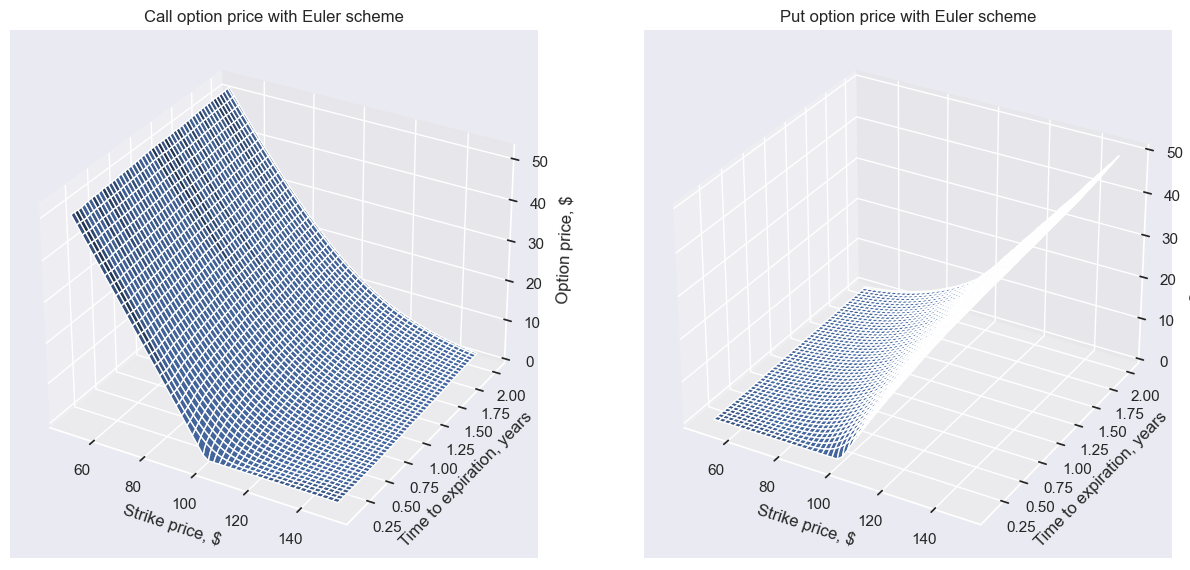
\includegraphics[width=\textwidth]{assets/euler.png}
        \end{figure}
    \end{frame}

    \begin{frame}{}
        \begin{figure}
            \centering
            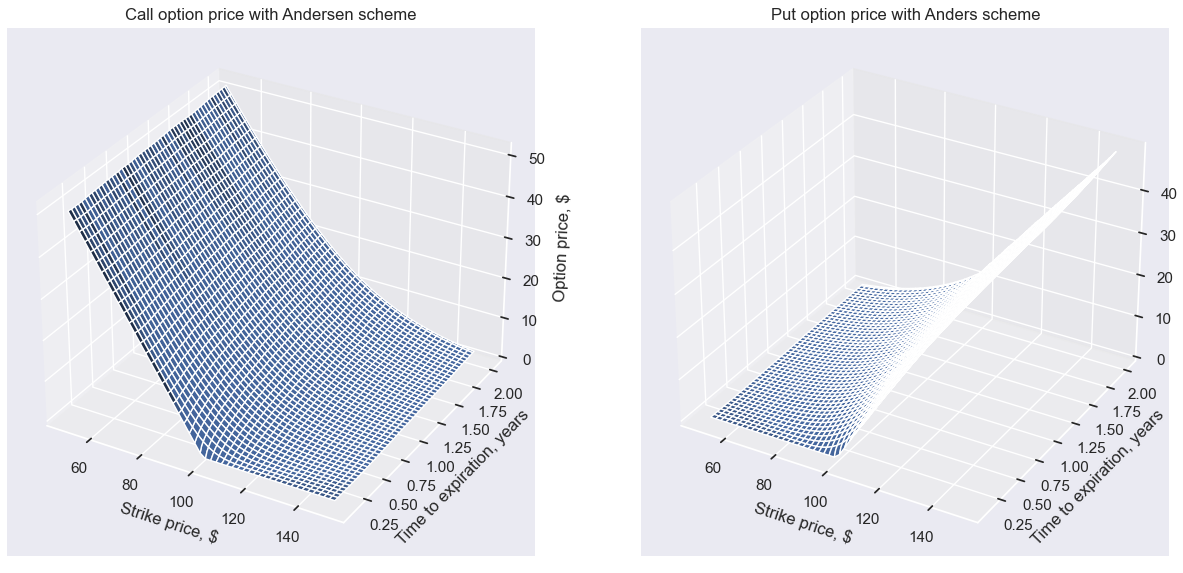
\includegraphics[width=\textwidth]{assets/andersen.png}
        \end{figure}
    \end{frame}

    \begin{frame}{}
        \begin{figure}
            \centering
            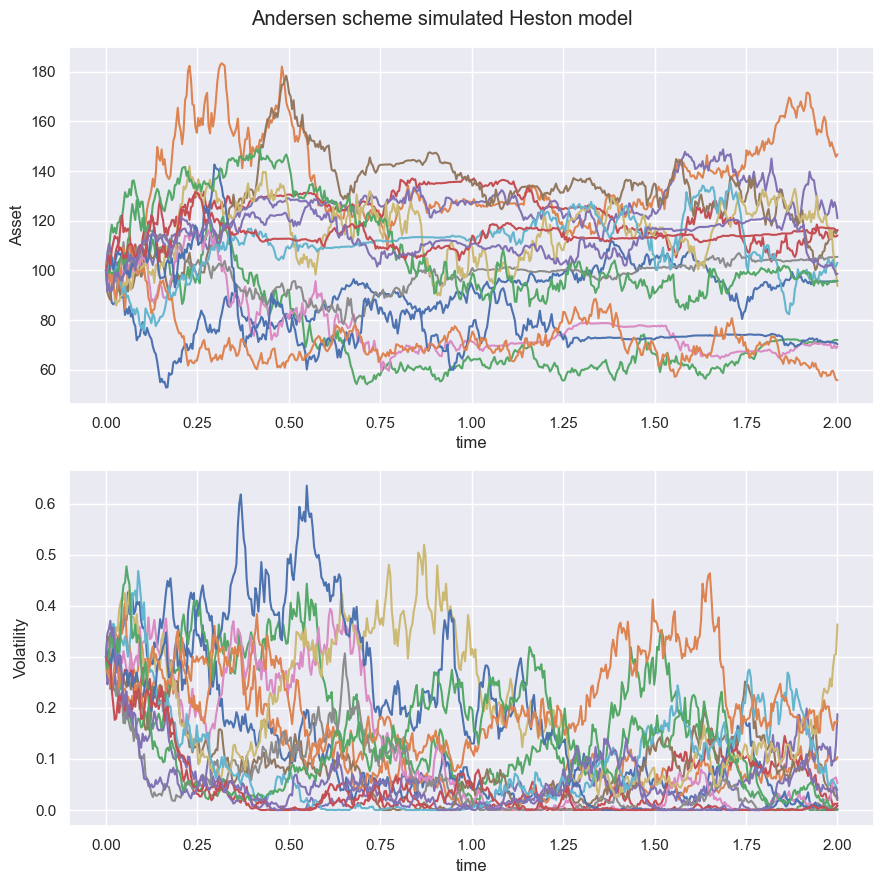
\includegraphics[width=0.65\textwidth]{assets/andersen_sim.png}
        \end{figure}
    \end{frame}

    \section{Greeks Computation}
        \begin{frame}{Conclusion}
    \begin{enumerate}
        \item We introduced the three common Heston simulation methods: Euler-Maruyama, Andersen TG and Andersen QE; 
        \item We compared the theoretical vanilla options prices and their Monte-Carlo counterparts;
        \item We measured the performance while pricing the exotics.
    \end{enumerate}
\end{frame}

\begin{frame}{To-dos}
    \begin{enumerate}
        \item Implement the Exact (Broadie and Kaya) scheme;
        \item Measure the preciseness of the pricers for the real market data;
        \item Estimate the discretization convergence order via RLS.
    \end{enumerate}
\end{frame}

    
    \section{Conclusion}
        \begin{frame}{Conclusion}
            We introduced the three most common simulation methods for dynamics of the Heston stochastic volatility model:
            \begin{enumerate}
                \item Euler scheme; \\
                \item Broadie-Kaya scheme; \\
                \item Andersen scheme.
            \end{enumerate}
        \end{frame}

\end{document}
